% Section content template for individual Educative lessons
% This file contains the actual content for a specific section
% Generated from Educative API section content

% Section: Getting Ready: The Facebook System
% Section ID: 5513562525270016
% Section Slug: getting-ready-the-facebook-system
% Generated: 2025-12-14T12:38:25.924154

\subsection{Problem definition}\label{8mWjBBkzQ_msT38LKJm8y-1}
\\
\textbf{Facebook} is a social media platform for users to connect with people and engage with different types of media and content. Users can connect with others by sending friend requests or using the direct messaging feature. Each user has a profile where they can create posts to share with their friends. Facebook also allows its users to create pages regarding a topic of interest and groups to form a community of similar people. Facebook generates a personalized feed for its users based on their friends, liked pages, groups, and the content they engage with to ensure the best experience.

\begin{figure}[htbp]
 \centering
 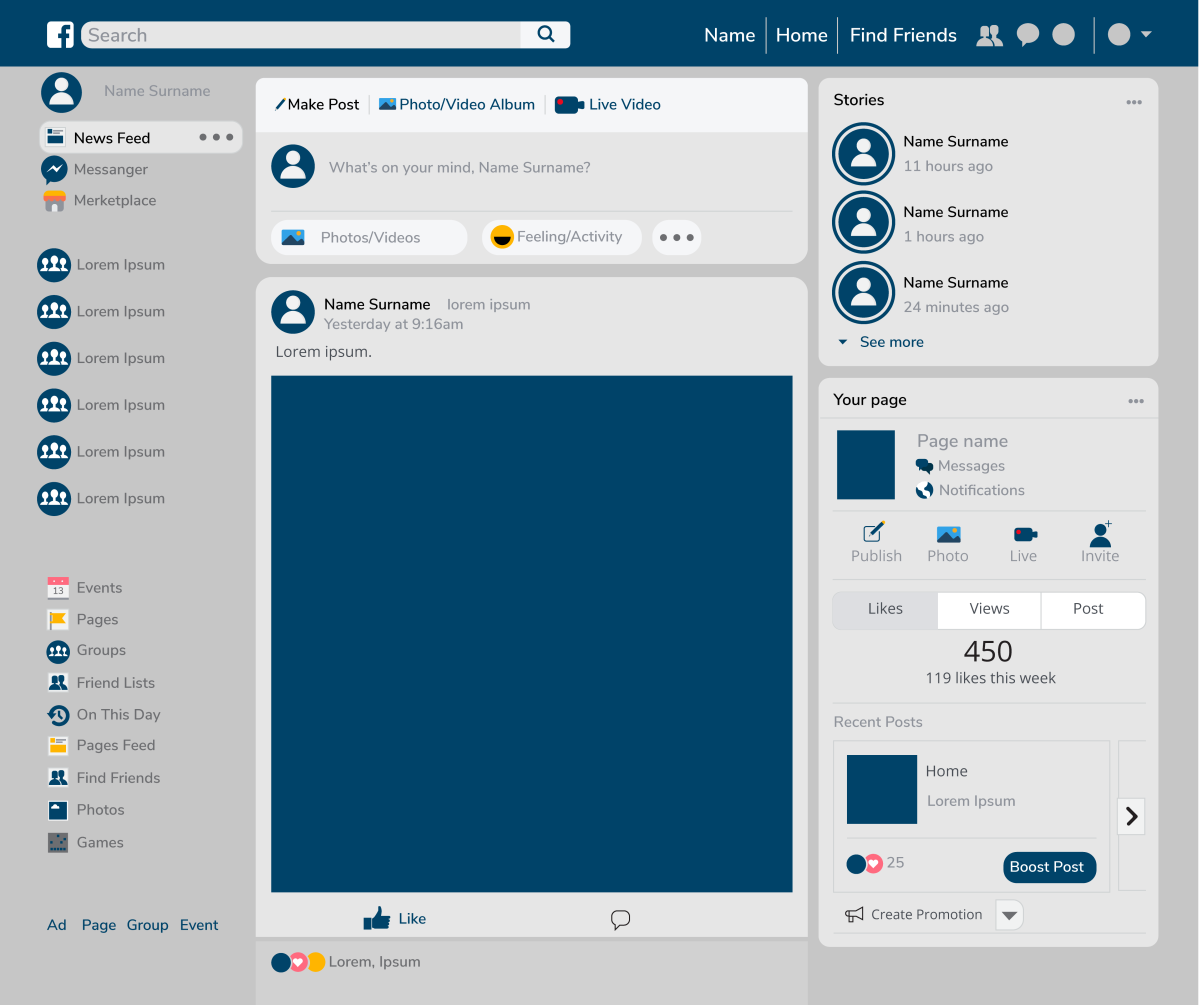
\includegraphics[width=0.5\textwidth]{Images/chapter_22/section_5513562525270016/6492547796172800.png}
 \caption{The Facebook home page of a user}
\end{figure}

\subsection{Expectations from the interviewee}\label{8mWjBBkzQ_msT38LKJm8y-2}
\\
Facebook offers multiple functionalities to its users. It is important to narrow down what components you will include in your Facebook design. The section below provides an overview of some of the main expectations the interviewer will want to hear you discuss in more detail.

\subsubsection{Discoverability}\label{c91yxLsvjn7uAcn3d1mrt}
\\
Developing a better understanding of how Facebook's discoverability works is important. The interviewer would expect you to ask the questions listed below:

\begin{itemize}
\item
\protect\phantomsection\label{qtrqwBpLByXHhU4AoCMAK}
How are users able to search other users' profiles?
\item
\protect\phantomsection\label{b--EwcroBVhKwmtfrs3N3}
Can users search other users using their phone numbers and email addresses?
\end{itemize}

\subsubsection{Friends and following}\label{VGR7ClzwPPl64nVfMA23v}
\\
The ``Add friend'' feature of Facebook is its most renowned feature. Make sure to ask the interviewer the questions provided below:

\begin{itemize}
\item
\protect\phantomsection\label{bKOJKgzsVt3Eo580sdZtL}
How are users able to add other users as friends?
\item
\protect\phantomsection\label{FcYedL5AtyaasR9gKUeiF}
How can users follow or unfollow other users without becoming a direct connection?
\end{itemize}

\subsubsection{Groups and pages}\label{O_yAGdn6DNBBzLuecZp-s}
\\
Groups and pages on Facebook create a space for like-minded individuals. Make sure to define your requirements. You may ask the interviewer the questions listed below:

\begin{itemize}
\item
\protect\phantomsection\label{G8oYUK08G_HtZqggOCbwu}
How can users create groups and pages besides their user profiles?
\item
\protect\phantomsection\label{euqbLSYNTPVBCprgztjyZ}
What are the criteria for joining a group? Can a user join a group if they are not friends with the creator of the group?
\end{itemize}

\subsubsection{Privacy}\label{o3TTODJfFMDBeNqrQlqV4}
\\
You can ask the following questions to learn about the privacy feature in your design:

\begin{itemize}
\item
\protect\phantomsection\label{H2j61vMfOMuzXArJ9tOBY}
How will the system handle privacy lists with certain content displayed only to specified connections?
\item
\protect\phantomsection\label{Ul9n4tlmbg_68VR9Tnj5Q}
How do users set the privacy of groups? How does this change the way members and non-members interact with the group?
\end{itemize}

\subsubsection{Alerts}\label{kzWHQSZX_PNtO897HE1Rv}
\\
Notifications and alerts allow users to stay updated with the activity in their circle. Therefore, you may want to understand how alerts will work in your system. You may ask the questions listed below:

\begin{itemize}
\item
\protect\phantomsection\label{ZWeuBiOu4LESPz3OEq_4a}
How will users be notified of pre-selected events?
\item
\protect\phantomsection\label{bwjonxEbYNNZpz5w6aq6E}
How much control do users have in choosing what notifications they can receive?
\end{itemize}

\subsection{Design approach}\label{VQfLJBfYFU2JanMuti5ND}
\\
We'll design Facebook using the bottom-up design approach. For this purpose, we will follow the steps below:

\begin{itemize}
\item
\protect\phantomsection\label{MchfvGRkeLfdZJ3-9fs2t}
Identify and design the smallest components, like a post and comment, first.
\item
\protect\phantomsection\label{RDEIXVmvWAZttt5SedON-}
Use these small components to design bigger components, for example, pages, groups, and profiles.
\item
\protect\phantomsection\label{gcAa9-H9BDofY-TsEiFlD}
Repeat the steps above until we design the complete Facebook platform.
\end{itemize}

\subsection{Design pattern~}\label{PLRSQybk-sqG3V2A6v2vu}
\\
During an interview, it is always a good practice to discuss the design patterns that Facebook follows. Stating the design patterns gives the interviewer a positive impression and shows that the interviewee is well-versed in the advanced concepts of object-oriented design.
\\
Try to answer the following question. If you are not familiar with design patterns, don't worry! You can learn about them by asking, ``Define design patterns.''

\textbf{Question:}

Which design pattern(s) should be used to design the Facebook system? Please elaborate on your choice(s).

Let's explore the requirements of Facebook in the next lesson.

% End of section content